No sistema de refrigeração, o evaporador é a parte onde o resfriamento do meio ocorre. Isso se dá pelo processo em que o refrigerante, na forma líquida, ao passar por essa região, absorve o calor do meio e assim evapora transformando-se em gás novamente. 
\begin{figure}[!htbp]
	 \centering
	  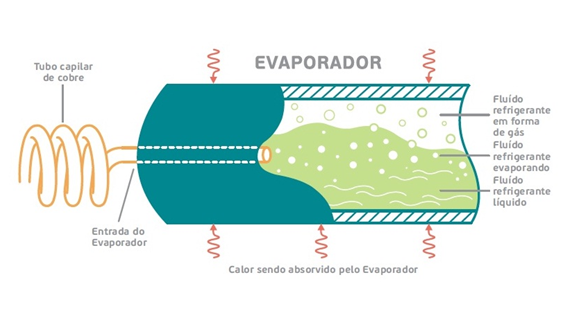
\includegraphics[scale=1]{editaveis/figuras/evaporador}
	  \caption[Esquema de processo de evaporação de o refrigerante]{Esquema de processo de evaporação de o refrigerante\footnotemark}
	  \label{condensador}
	\end{figure}	   
	\footnotetext{Disponível em: http://www.clubedarefrigeracao.com.br/material/colecao-tecnica}
	\FloatBarrier
	
	
Basicamente, existem alguns tipos de evaporadores e eles variam de acordo com a disposição ou necessidade. O evaporador de do tipo placa (roll-bond) é muito comum nas casas brasileiras, já que pode ser encontrado nos refrigeradores domésticos. Ele é composto por duas chapas de alumínio sobrepostas e entre elas um tubulação em forma de ziguezague por onde passa o refrigerante. Outro tipo bem parecido é o tubular, que apresenta uma serpentina colada em uma placa de alumínio.\cite{embracocolecao}.

O evaporador aletado apresenta um tubo de alumínio com aletas de alumínio \cite{embracocolecao}. Diferente dos dois tipos apresentados no paragrafo anterior, esse aveporador, tambem chamado de evaporador de ar forçado, precisa de um ventilador que possa movimentar o ar para dentro e assim ter uma maior vazão. 

Com essa análise, foi escolhido o evaporador de ar forçado, visto que, em caso de haver pouco vento ou variação do mesmo na região de Acarí, a produção de água não seria prejudicada já que os ventiladores serviram para manter um fluxo constante de entrada de ar para que a produção de água fique dentro das metas já pré-estabelecidas. 
Outra justificativa para escolha desse tipo de evaporador é que ele se adequa as restrições feitas pelos cálculos no Anexo A, que definem a vazão necessária para que ocorra a produção da quantidade de água prevista pelo escopo.

O fabricante do evaporador escolhido foi a TrinevaTM, principalmente porque eles trabalham com evaporadores de alta vazão e, por ser um fabricante nacional, tornará o custo do produto e do frete mais acessíveis em relação à um fabricante no exterior. 

\begin{figure}[!htbp]
	 \centering
	  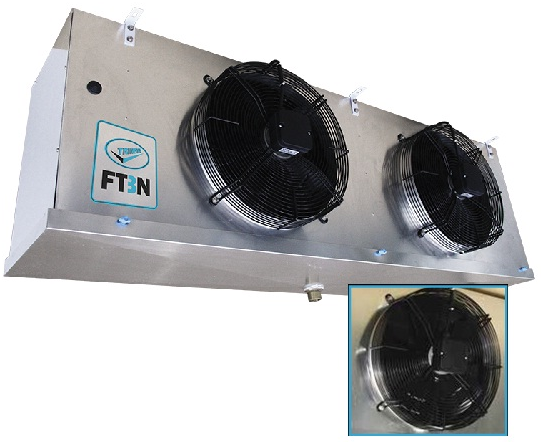
\includegraphics[scale=1]{editaveis/figuras/evaporador_trivena}
	  \caption[Evaporador trivena]{Evaporador Trineva\textsuperscript{TM} da linha FTBN e, em detalhe, o motoventilador de 400mm com rotor externo \footnotemark}
	  \label{evaporador}
	\end{figure}	   
	\footnotetext{Disponível em: http://trineva.com.br/?page\_id=122}
	\FloatBarrier
	
Essas dimensões apresentadas podem ser atribuídas as seguintes cotas da imagem abaixo.
\begin{figure}[!htbp]
	 \centering
	  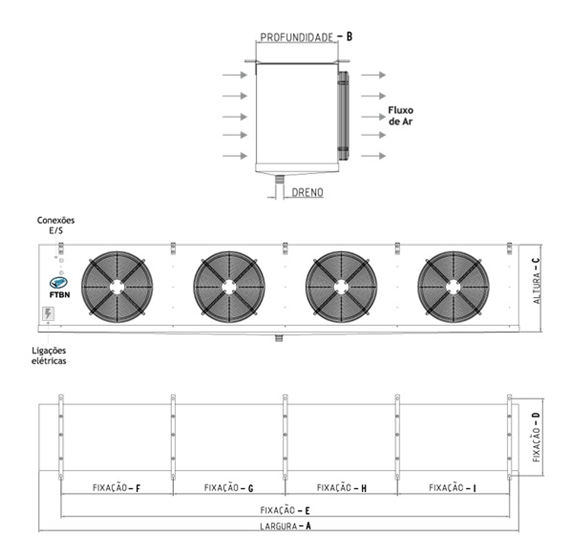
\includegraphics[scale=1]{editaveis/figuras/cotas_evaporador}
	  \caption[Cotas evaporador]{Cotas das três vistas ortográficas do modelo geral de evaporador \footnotemark}
	  \label{cota_evaporador}
	\end{figure}	   
	\footnotetext{Disponível em: http://trineva.com.br/?page\_id=122}
	\FloatBarrier
	
O desempenho térmico e a vazão do evaporador escolhido estão dentro do quadro amarelo da imagem que se segue.
\begin{figure}[!htbp]
	 \centering
	  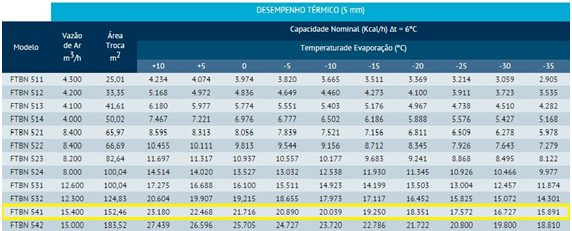
\includegraphics[scale=1]{editaveis/figuras/desenho_termico}
	  \caption[Vazão do evaporador]{Vazão do evaporador, assim como sua área e desempenho térmico \footnotemark}
	  \label{vazao_evaporador}
	\end{figure}	   
	\footnotetext{Disponível em: http://trineva.com.br/?page\_id=122}
	\FloatBarrier
	
Para os ventiladores e o sistema de degelo, a Trineva\textsuperscript{TM} fornece os seguintes dados para o modelo escolhido:
\begin{figure}[!htbp]
	 \centering
	  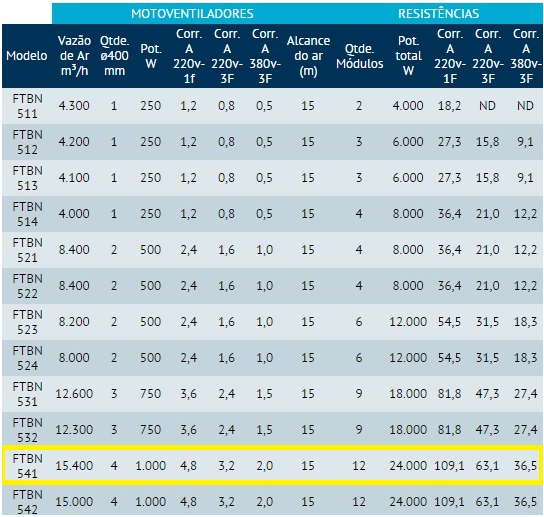
\includegraphics[scale=1]{editaveis/figuras/dados_ventiladores}
	  \caption[Dados dos ventiladores]{Dados dos ventiladores e das resistências elétricas \footnotemark}
	  \label{vazao_evaporador}
	\end{figure}	   
	\footnotetext{Disponível em: http://trineva.com.br/?page\_id=122}
	\FloatBarrier